\documentclass[12pt,a4paper]{report}

\usepackage[utf8]{inputenc}
\usepackage[T1]{fontenc}
\usepackage[french]{babel}
\usepackage{geometry}
\usepackage{graphicx}
\usepackage{float}
\usepackage{array}
\usepackage{longtable}
\usepackage{booktabs}
\usepackage{hyperref}
\usepackage{xcolor}
\usepackage{listings}
\usepackage{setspace}
\usepackage[nobottomtitles*]{titlesec}
\usepackage{fancyhdr}
\usepackage{enumitem}
\usepackage{needspace}
\usepackage{colortbl}

\geometry{left=2.5cm,right=2.5cm,top=2.5cm,bottom=2.5cm}
\onehalfspacing
\setlength{\parindent}{0.7cm}
\setlength{\parskip}{0.25cm}

\definecolor{primaryblue}{HTML}{1E3A8A}
\definecolor{softgray}{HTML}{F3F4F6}
\definecolor{codegray}{HTML}{111827}

\hypersetup{
    colorlinks=true,
    linkcolor=primaryblue,
    urlcolor=primaryblue,
    citecolor=primaryblue,
    pdftitle={Rapport de Projet de Fin d'Etudes - EduFlow},
    pdfauthor={Etudiant}
}

\lstset{
    basicstyle=\ttfamily\small,
    breaklines=true,
    frame=single,
    backgroundcolor=\color{softgray},
    rulecolor=\color{primaryblue},
    columns=fullflexible,
    keywordstyle=\color{primaryblue},
    commentstyle=\color{gray},
    stringstyle=\color{codegray}
}

\pagestyle{fancy}
\fancyhf{}
\lhead{EduFlow}
\rhead{Projet de fin d'études}
\cfoot{\thepage}

\titleformat{\chapter}[display]
{\normalfont\huge\bfseries\color{primaryblue}}
{\chaptertitlename\ \thechapter}
{20pt}
{\Huge}

\begin{document}

\begin{titlepage}
    \centering
    \vspace*{0.5cm}
    {\large \textbf{OFPPT / CMC CASABLANCA – SETTAT}}\\[0.2cm]
    {\large Filière : Développement Digital — Web Full Stack}\\[1.5cm]

    {\Large \textbf{Rapport de Projet de Fin d'Études}}\\[1cm]

    {\Huge \textbf{EduFlow}}\\[0.4cm]
    {\Large Système web de gestion financière et administrative scolaire}\\[1.5cm]

    \rule{0.85\textwidth}{0.5pt}\\[0.8cm]
    {\large Application SaaS de gestion financière scolaire \\ (Architecture Multi-tenant Web Full Stack)}\\[0.8cm]
    \rule{0.85\textwidth}{0.5pt}\\[2cm]

    \begin{tabular}{rl}
        \textbf{Réalisé par :} & \textit{Salma RAHIB} \\
        \textbf{Encadrant :} & \textit{M. GOUMIH Mohamed} \\
        \textbf{Année de formation :} & \textit{2025--2026} \\
    \end{tabular}

    \vfill
    {\large Année de Formation : 2025--2026}
\end{titlepage}

\pagenumbering{roman}

\chapter*{Dédicace}
\addcontentsline{toc}{chapter}{Dédicace}

Je dédie ce travail à ma famille, pour son soutien moral et ses encouragements tout au long de mon parcours. Je le dédie également à mes enseignants et à toutes les personnes qui ont contribué, directement ou indirectement, à ma formation et à la réussite de ce projet.

\chapter*{Remerciements}
\addcontentsline{toc}{chapter}{Remerciements}

Avant tout, je rends grâce à Allah, le Tout-Puissant, de m'avoir accordé la santé, la force et la persévérance nécessaires pour mener à bien ce projet de fin d'études.

J'adresse mes plus sincères remerciements à \textbf{Monsieur GOUMIH Mohamed}, mon encadrant pédagogique, pour son accompagnement, sa disponibilité et ses précieux conseils tout au long de la réalisation de ce projet. Je lui suis reconnaissante pour sa confiance, sa rigueur, ses orientations et ses remarques constructives, qui m'ont permis d'améliorer la qualité de mon travail et d'approfondir mes compétences.

Je remercie également l'ensemble de l'équipe pédagogique du \textbf{CMC Casablanca–Settat} pour la qualité de la formation dispensée, leur professionnalisme et leur engagement, qui m'ont permis d'acquérir de solides connaissances en développement informatique.

Mes remerciements s'adressent également aux membres du jury pour le temps consacré à l'évaluation de ce travail ainsi que pour leurs remarques et recommandations.

Enfin, j'exprime toute ma gratitude à ma famille, à mes amis ainsi qu'à toutes les personnes qui m'ont soutenue, encouragée et accompagnée de près ou de loin durant cette expérience. Leur confiance et leurs encouragements ont été une véritable source de motivation tout au long de ce parcours.

\chapter*{Résumé}
\addcontentsline{toc}{chapter}{Résumé}

EduFlow est une application web destinée à la gestion financière et administrative d'un établissement scolaire. Elle permet de gérer les élèves, les classes, les mensualités, les paiements, les impayés, les utilisateurs et les écoles. Le système repose sur une architecture client-serveur composée d'une interface frontend développée avec React, d'une API REST développée en PHP natif, et d'une base de données MySQL.

Le projet met en œuvre plusieurs concepts importants du développement logiciel : authentification par jeton JWT, contrôle d'accès par rôle, conception d'API REST, modélisation relationnelle des données, séparation des responsabilités côté backend, routage côté frontend et déploiement local avec Docker. L'objectif principal est de proposer une solution claire, pratique et évolutive pour simplifier le suivi financier des établissements scolaires.

\textbf{Mots-clés :} gestion scolaire, finance scolaire, React, PHP, MySQL, JWT, API REST, Docker.

\tableofcontents
\listoffigures
\listoftables

\clearpage
\pagenumbering{arabic}

\chapter*{Introduction générale}
\addcontentsline{toc}{chapter}{Introduction générale}

La gestion administrative et financière d'un établissement scolaire représente une activité essentielle, mais souvent complexe. Elle implique le suivi des élèves, des classes, des frais mensuels, des paiements, des retards de paiement, des utilisateurs et des droits d'accès. Dans plusieurs petites et moyennes structures, ces opérations sont encore réalisées manuellement à l'aide de feuilles de calcul, de documents papier ou d'outils non centralisés. Cette situation peut provoquer des erreurs, des pertes de temps, des difficultés de suivi et un manque de visibilité sur l'état financier réel de l'établissement.

Dans ce contexte, le projet EduFlow propose une solution web centralisée permettant de faciliter la gestion financière scolaire. L'application offre une interface moderne pour les utilisateurs et une API backend structurée pour la gestion des données. Elle permet aux administrateurs de suivre les paiements, d'identifier les impayés, de gérer les élèves et d'obtenir une vue synthétique grâce aux tableaux de bord.

Ce rapport présente l'ensemble du travail réalisé, depuis l'étude du besoin jusqu'à la mise en œuvre technique. Il décrit le contexte du projet, l'analyse fonctionnelle, la conception UML, l'architecture logicielle, les technologies utilisées, les principales fonctionnalités, les tests réalisés ainsi que les perspectives d'amélioration.

\chapter{Présentation du projet}

\section{Contexte général}

La digitalisation des services administratifs est devenue un élément important pour améliorer la qualité de gestion au sein des établissements scolaires. Les écoles doivent aujourd'hui gérer un volume important d'informations : élèves, parents, classes, utilisateurs, paiements et rapports financiers. Lorsque ces informations sont dispersées, l'administration devient plus lente et moins fiable.

EduFlow s'inscrit dans cette logique de transformation numérique. Le projet vise à offrir une plateforme web simple à utiliser, capable de centraliser les principales opérations liées à la gestion financière scolaire.

\section{Problématique}

La problématique principale peut être formulée ainsi :

\begin{quote}
Comment concevoir et développer une application web permettant à un établissement scolaire de gérer efficacement ses élèves, ses paiements mensuels, ses impayés et ses utilisateurs, tout en garantissant la sécurité des accès et la fiabilité des données ?
\end{quote}

Cette problématique se décline en plusieurs difficultés :

\begin{itemize}[label=--]
    \item le suivi manuel des paiements est lent et sujet aux erreurs ;
    \item l'identification des impayés demande souvent un travail répétitif ;
    \item les données des élèves et des parents peuvent être dispersées ;
    \item les droits d'accès ne sont pas toujours clairement définis ;
    \item les responsables ont besoin d'indicateurs simples pour prendre des décisions.
\end{itemize}

\section{Objectifs du projet}

Les objectifs principaux du projet sont les suivants :

\begin{itemize}[label=--]
    \item développer une application web de gestion financière scolaire ;
    \item permettre l'authentification sécurisée des utilisateurs ;
    \item gérer les rôles \texttt{super\_admin}, \texttt{admin} et \texttt{user} ;
    \item gérer les élèves, les classes et les écoles ;
    \item suivre les mensualités, les paiements et les montants restants ;
    \item afficher les impayés de manière claire ;
    \item proposer des tableaux de bord pour le suivi financier ;
    \item structurer le code pour faciliter la maintenance et l'évolution.
\end{itemize}

\section{Périmètre du projet}

Le périmètre fonctionnel d'EduFlow couvre les modules suivants :

\begin{itemize}[label=--]
    \item authentification et gestion de session ;
    \item gestion des utilisateurs et des rôles ;
    \item gestion des écoles par le super administrateur ;
    \item gestion des élèves et des classes ;
    \item gestion des mensualités ;
    \item enregistrement et suivi des paiements ;
    \item consultation des impayés ;
    \item tableaux de bord administratifs ;
    \item génération ou consultation des reçus.
\end{itemize}

\chapter{Analyse des besoins}

\section{Acteurs du système}

Le système distingue plusieurs acteurs, chacun disposant de droits spécifiques.

\begin{longtable}{|p{4cm}|p{10cm}|}
\hline
\textbf{Acteur} & \textbf{Description} \\
\hline
Visiteur & Personne non authentifiée pouvant accéder uniquement à la page de connexion. \\
\hline
Utilisateur & Utilisateur rattaché à une école, disposant d'un accès limité aux fonctionnalités opérationnelles. \\
\hline
Administrateur & Responsable d'une école pouvant gérer les élèves, les classes, les paiements, les utilisateurs et les données financières. \\
\hline
Super administrateur & Responsable global de la plateforme pouvant gérer les écoles, les administrateurs et les tableaux de bord globaux. \\
\hline
\caption{Acteurs principaux du système}
\end{longtable}

\section{Besoins fonctionnels}

\begin{longtable}{|p{4cm}|p{10cm}|}
\hline
\textbf{Module} & \textbf{Besoins fonctionnels} \\
\hline
Authentification & Connexion par email et mot de passe, génération d'un jeton JWT, protection des routes privées. \\
\hline
Gestion des élèves & Ajouter, modifier, supprimer et consulter les élèves avec leurs informations scolaires et financières. \\
\hline
Gestion des classes & Créer et lister les niveaux de classe, organiser les élèves selon leur classe. \\
\hline
Mensualités & Consulter les frais mensuels, identifier les statuts payés, partiels ou impayés. \\
\hline
Paiements & Enregistrer les paiements, consulter l'historique et associer un paiement à une mensualité. \\
\hline
Impayés & Afficher les frais non payés ou partiellement payés afin de faciliter le suivi administratif. \\
\hline
Tableaux de bord & Afficher des indicateurs financiers, les paiements récents et les montants à recouvrer. \\
\hline
Administration des écoles & Créer et gérer les écoles, affecter des administrateurs et gérer les informations générales. \\
\hline
Gestion des utilisateurs & Créer, consulter et modifier les utilisateurs selon les autorisations du rôle connecté. \\
\hline
\caption{Besoins fonctionnels}
\end{longtable}

\section{Besoins non fonctionnels}

\begin{itemize}[label=--]
    \item \textbf{Sécurité :} les mots de passe sont stockés sous forme hachée et les accès sont protégés par JWT.
    \item \textbf{Fiabilité :} les données sont stockées dans une base relationnelle MySQL.
    \item \textbf{Maintenabilité :} le backend sépare les contrôleurs, services, modèles, middleware et composants du cœur.
    \item \textbf{Ergonomie :} l'interface frontend est organisée par pages et par navigation protégée.
    \item \textbf{Évolutivité :} la présence du champ \texttt{school\_id} permet une logique multi-écoles.
    \item \textbf{Portabilité :} la base de données peut être lancée localement avec Docker.
\end{itemize}

\section{Règles de gestion}

Les principales règles de gestion identifiées sont :

\begin{itemize}[label=--]
    \item un utilisateur doit être authentifié pour accéder aux modules internes ;
    \item certaines fonctionnalités sont limitées aux rôles \texttt{admin} et \texttt{super\_admin} ;
    \item seul le super administrateur peut gérer toutes les écoles ;
    \item un paiement est associé à un élève et à une mensualité ;
    \item une mensualité peut être payée, partiellement payée ou impayée ;
    \item les tableaux de bord présentent uniquement les informations autorisées pour le rôle connecté.
\end{itemize}

\chapter{Conception UML}

\section{Présentation}

La modélisation UML permet de représenter le système avant et pendant la phase de développement. Elle facilite la compréhension des acteurs, des fonctionnalités et des interactions principales. Le projet contient déjà des fichiers PlantUML dans le dossier \texttt{UML/}. Ces fichiers peuvent être exportés en images puis insérés dans ce rapport.

\section{Diagramme global}

\begin{figure}[H]
    \centering
    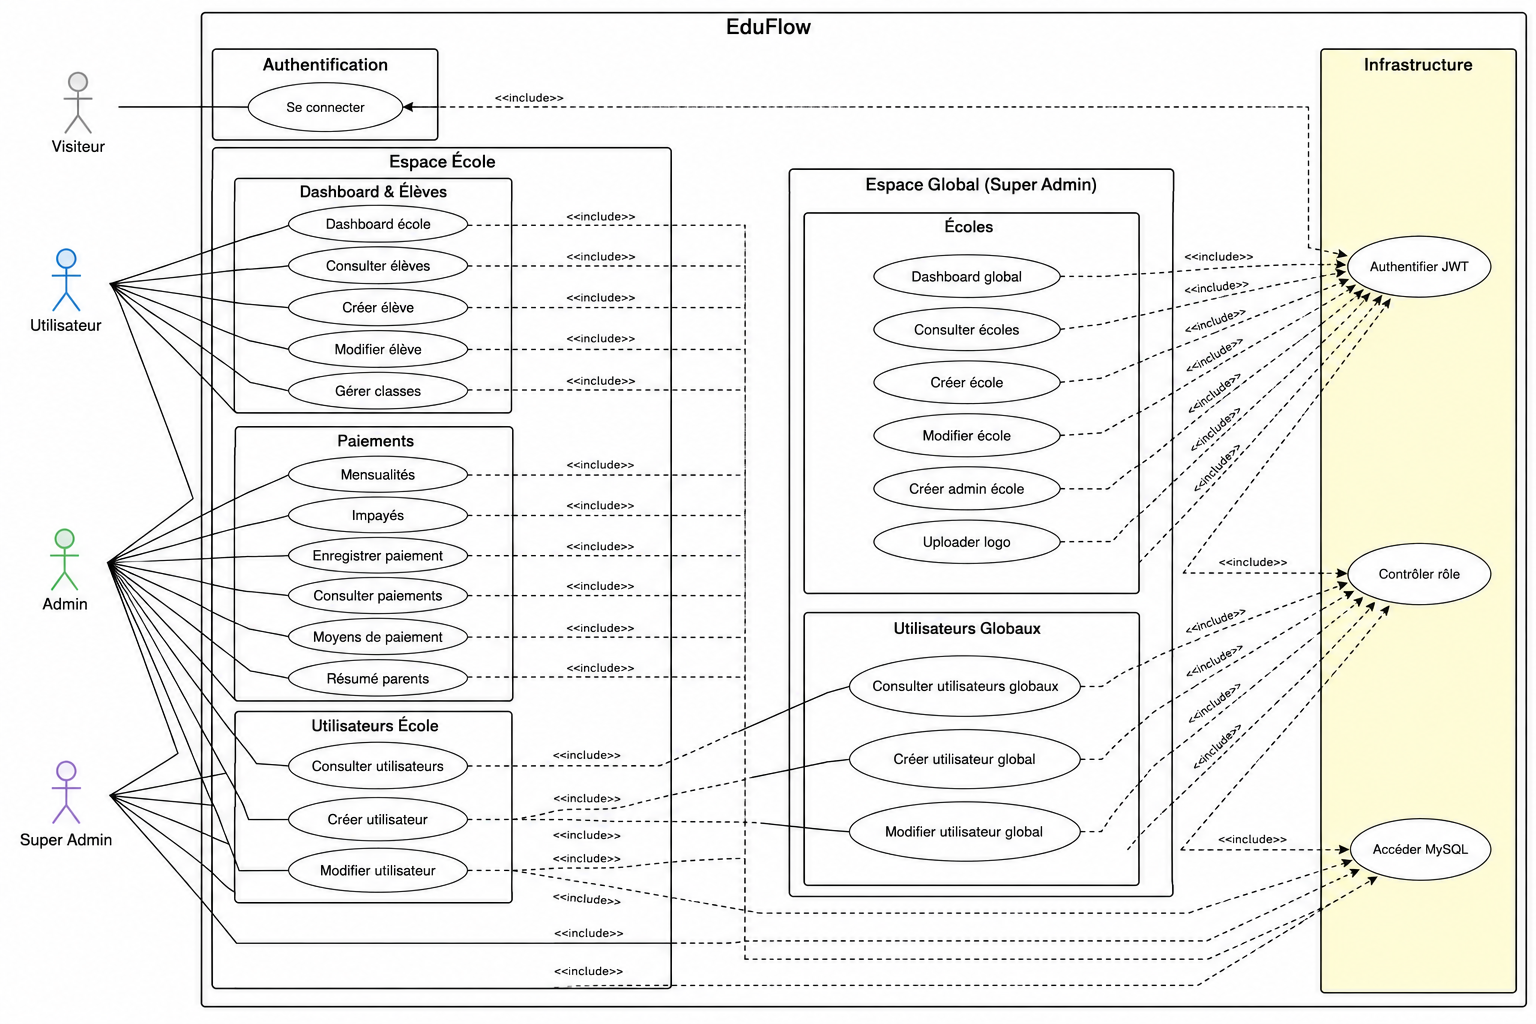
\includegraphics[width=0.9\textwidth]{UML/eduflow.png}
    \caption{Diagramme UML global du système EduFlow}
    \label{fig:uml-global}
\end{figure}

\section{Diagramme du visiteur}

\begin{figure}[H]
    \centering
    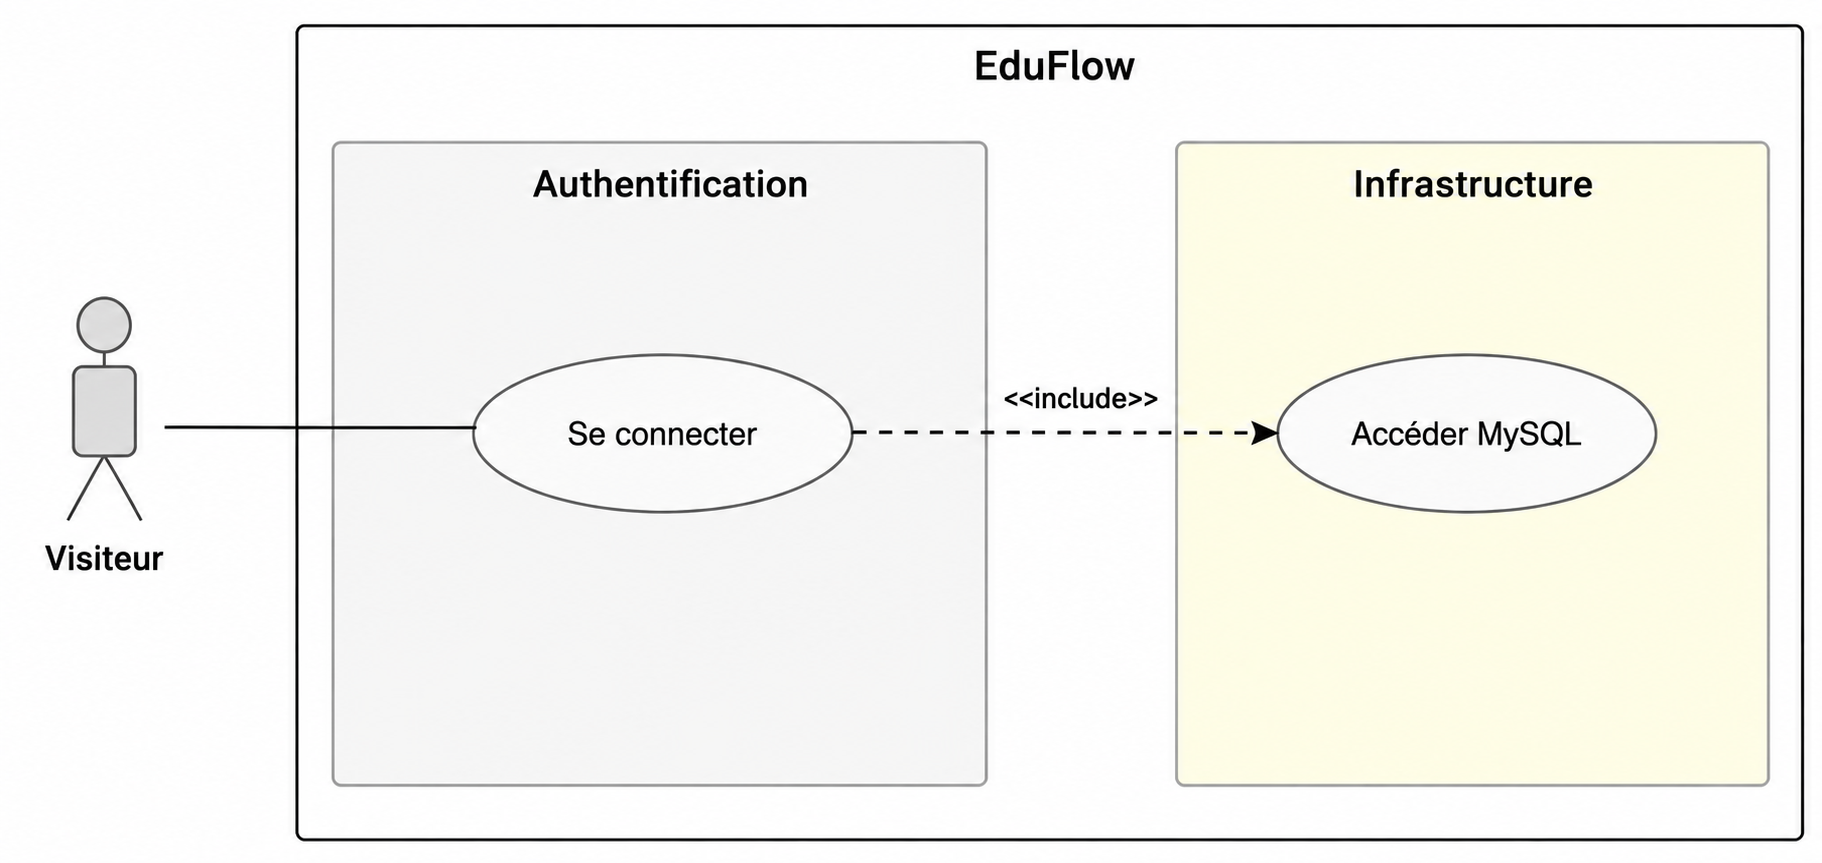
\includegraphics[width=0.85\textwidth]{UML/1_visitor.png}
    \caption{Diagramme de cas d'utilisation du visiteur}
    \label{fig:uml-visiteur}
\end{figure}

\section{Diagramme de l'utilisateur}

\begin{figure}[H]
    \centering
    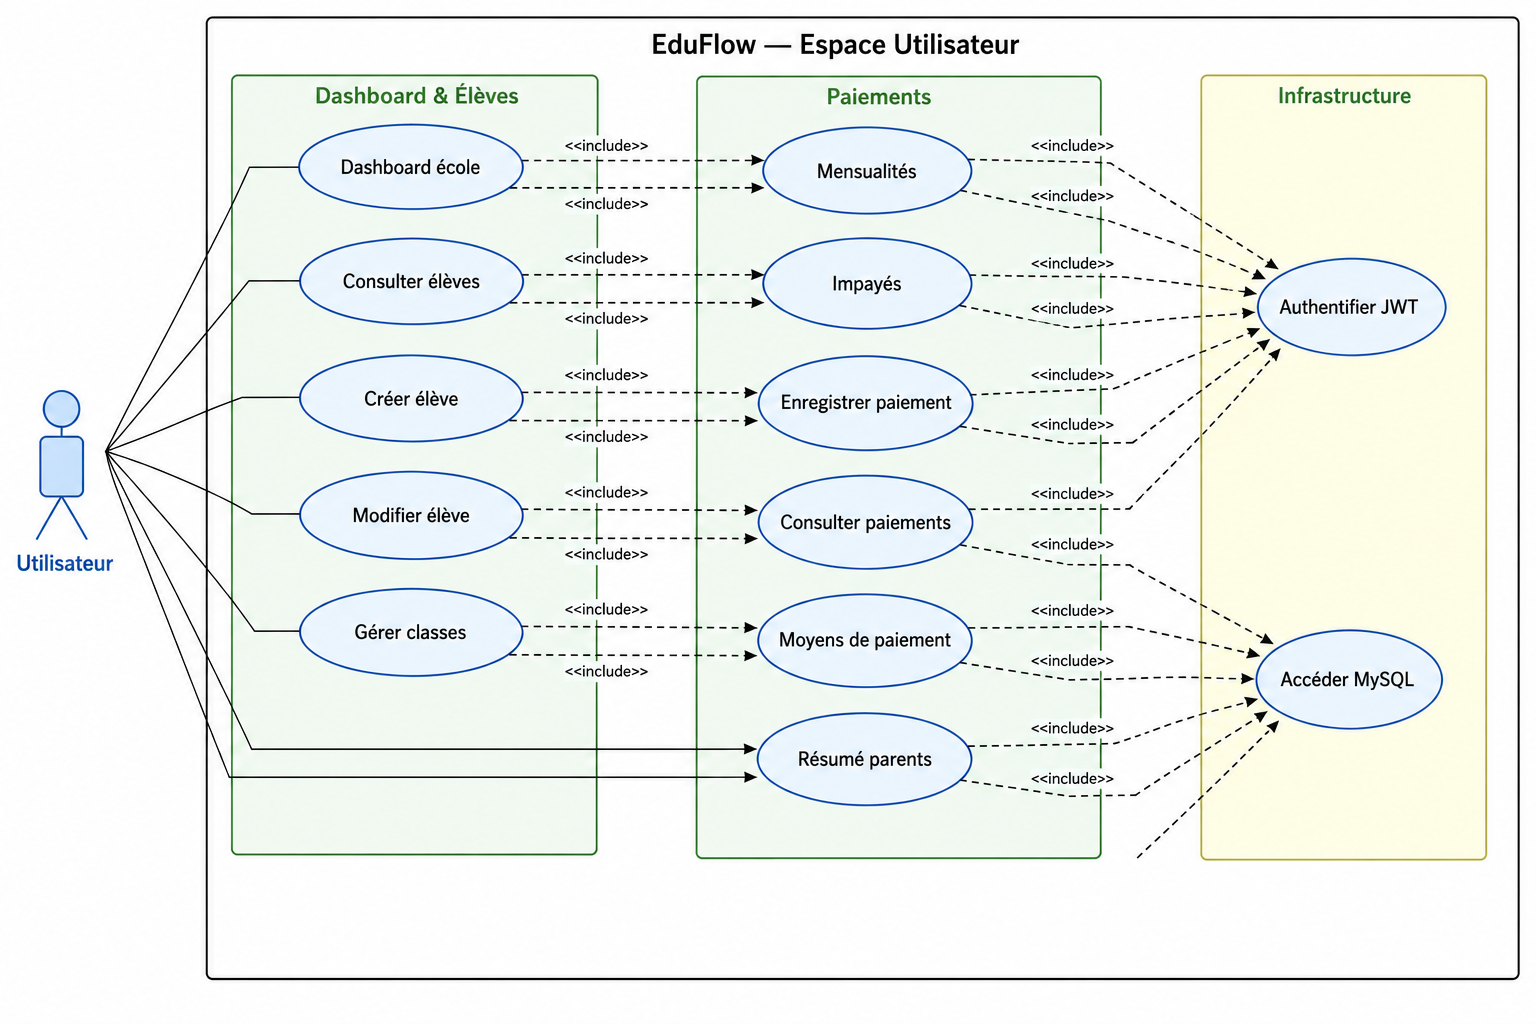
\includegraphics[width=0.85\textwidth]{UML/2_user.png}
    \caption{Diagramme de cas d'utilisation de l'utilisateur}
    \label{fig:uml-user}
\end{figure}

\section{Diagramme de l'administrateur}

\begin{figure}[H]
    \centering
    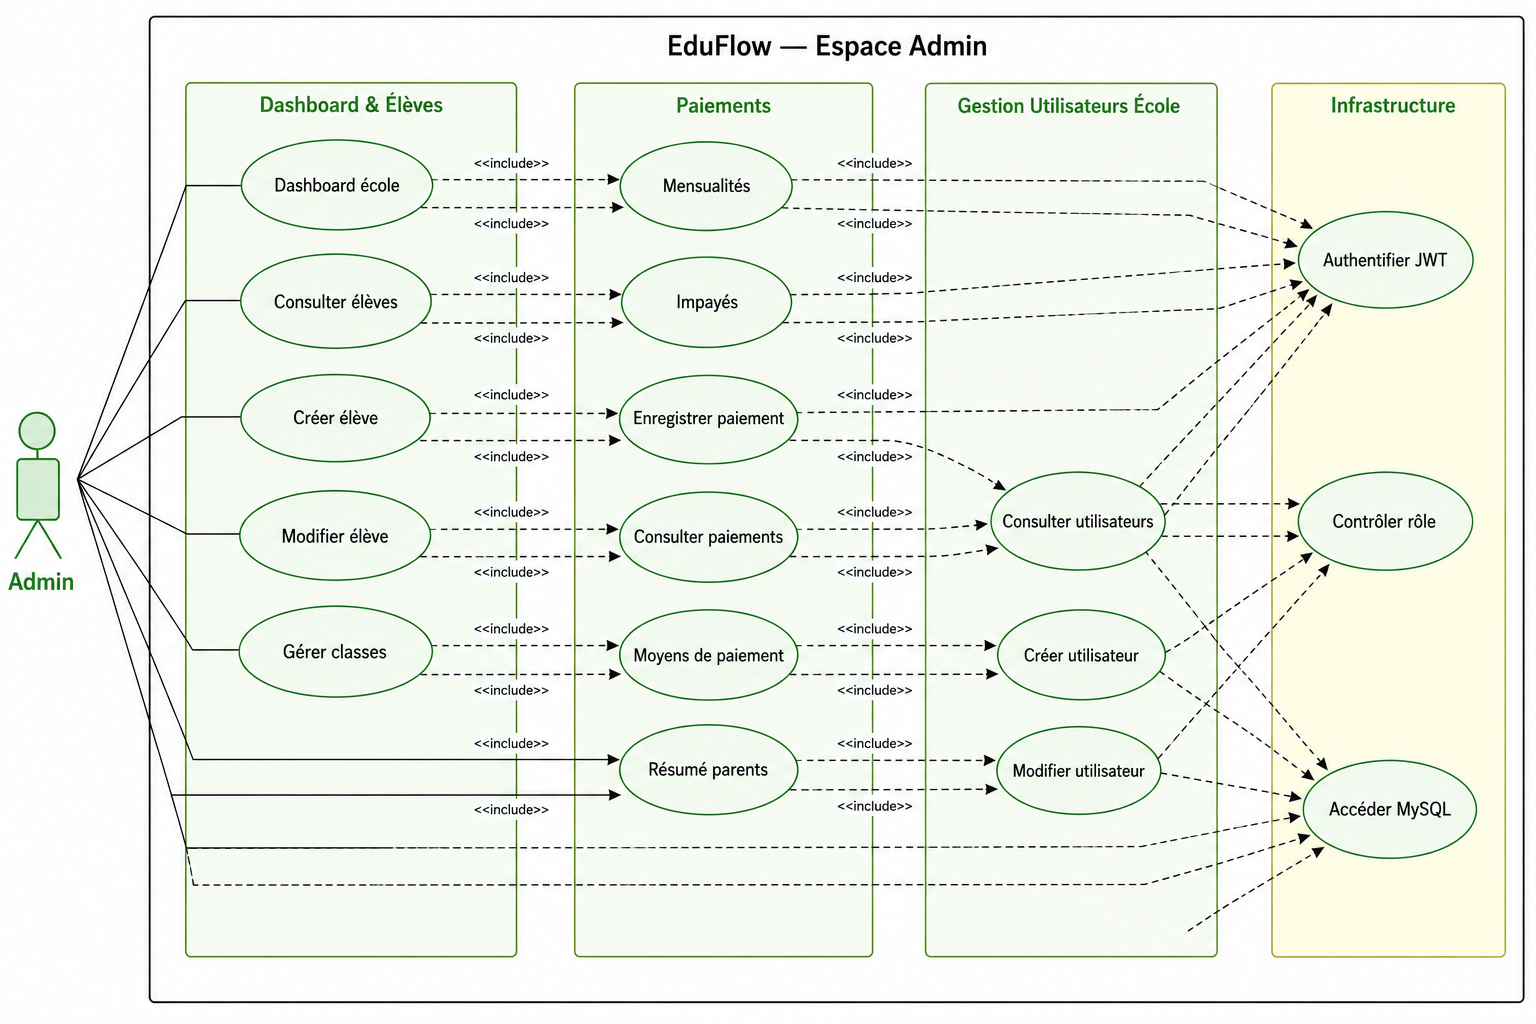
\includegraphics[width=0.85\textwidth]{UML/3_admin.png}
    \caption{Diagramme de cas d'utilisation de l'administrateur}
    \label{fig:uml-admin}
\end{figure}

\section{Diagramme du super administrateur}

\begin{figure}[H]
    \centering
    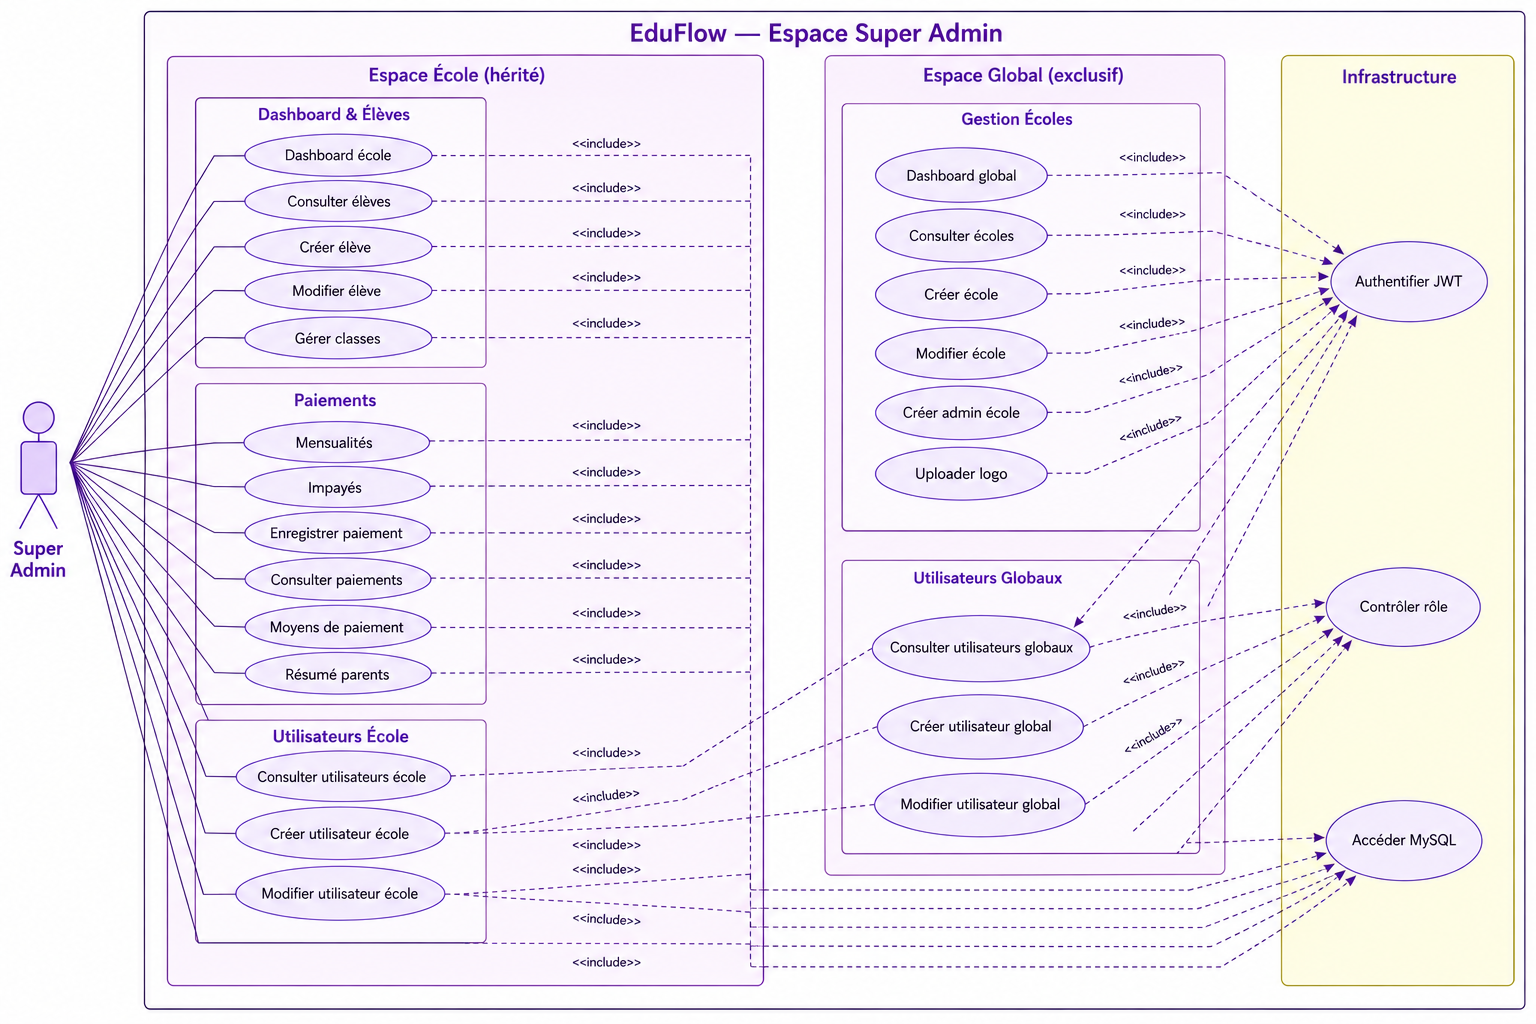
\includegraphics[width=0.85\textwidth]{UML/4_superadmin.png}
    \caption{Diagramme de cas d'utilisation du super administrateur}
    \label{fig:uml-superadmin}
\end{figure}

\chapter{Architecture technique}

\section{Architecture générale}

EduFlow repose sur une architecture client-serveur. Le client est une application React exécutée dans le navigateur. Le serveur est une API REST développée en PHP. Les données sont stockées dans une base MySQL. La communication entre le frontend et le backend se fait par des requêtes HTTP au format JSON.

\begin{figure}[H]
    \centering
    \fbox{\parbox{0.86\textwidth}{
        \centering
        \vspace{2cm}
        Navigateur React\\
        $\Downarrow$ Requêtes HTTP / JSON\\
        API REST PHP\\
        $\Downarrow$ PDO\\
        Base de données MySQL\\
        \vspace{2cm}
    }}
    \caption{Architecture générale de l'application}
    \label{fig:architecture-generale}
\end{figure}

\section{Architecture frontend}

Le frontend est développé avec React et Vite. Il est organisé autour de pages, de services, de contextes et de composants communs. Les routes sont protégées selon l'état d'authentification et le rôle de l'utilisateur.

\begin{itemize}[label=--]
    \item \texttt{src/pages} : contient les pages principales de l'application ;
    \item \texttt{src/services} : contient les services Axios pour appeler l'API ;
    \item \texttt{src/context} : gère le contexte d'authentification ;
    \item \texttt{src/routes} : définit les routes de navigation ;
    \item \texttt{src/components/common} : contient les composants de protection des routes.
\end{itemize}

\section{Architecture backend}

Le backend est développé en PHP natif avec une organisation inspirée des architectures en couches. Chaque couche possède une responsabilité précise.

\begin{longtable}{|p{4cm}|p{10cm}|}
\hline
\textbf{Dossier} & \textbf{Responsabilité} \\
\hline
\texttt{Controllers} & Réception des requêtes HTTP et préparation des réponses. \\
\hline
\texttt{Services} & Traitement de la logique métier. \\
\hline
\texttt{Models} & Représentation des entités principales et interaction avec les données. \\
\hline
\texttt{Middleware} & Vérification de l'authentification et des rôles. \\
\hline
\texttt{Core} & Routage, connexion à la base de données, gestion des requêtes, réponses et JWT. \\
\hline
\caption{Organisation du backend PHP}
\end{longtable}

\section{Architecture de la base de données}

La base de données contient plusieurs tables liées entre elles. Les tables principales sont :

\begin{itemize}[label=--]
    \item \texttt{schools} : informations des écoles ;
    \item \texttt{users} : utilisateurs et rôles ;
    \item \texttt{class\_levels} : niveaux ou classes ;
    \item \texttt{parents} : informations des parents ;
    \item \texttt{students} : élèves ;
    \item \texttt{monthly\_fees} : mensualités ;
    \item \texttt{payments} : paiements ;
    \item \texttt{payment\_methods} : méthodes de paiement.
\end{itemize}

\chapter{Réalisation}

\section{Technologies utilisées}

\begin{table}[H]
\centering
\begin{tabular}{|p{4cm}|p{9cm}|}
\hline
\textbf{Technologie} & \textbf{Utilisation dans le projet} \\
\hline
React & Construction de l'interface utilisateur. \\
\hline
Vite & Serveur de développement frontend et génération du build. \\
\hline
Axios & Communication HTTP avec l'API backend. \\
\hline
React Router & Gestion des routes côté frontend. \\
\hline
PHP 8 & Développement de l'API REST backend. \\
\hline
Composer & Gestion des dépendances PHP. \\
\hline
MySQL 8 & Stockage relationnel des données. \\
\hline
Docker & Exécution locale de la base MySQL. \\
\hline
JWT & Authentification par jeton. \\
\hline
\end{tabular}
\caption{Technologies utilisées}
\end{table}

\section{Authentification}

L'authentification constitue un élément central du système. Lorsqu'un utilisateur saisit son email et son mot de passe, le frontend envoie une requête vers l'endpoint \texttt{/api/login}. Le backend vérifie les informations dans la base de données. Si les identifiants sont valides, un jeton JWT est généré et retourné avec les informations de l'utilisateur.

Ce jeton est ensuite envoyé dans l'en-tête \texttt{Authorization} des requêtes protégées. Le middleware backend vérifie la validité du jeton et autorise ou refuse l'accès à la ressource demandée.

\section{Gestion des rôles}

Le projet distingue trois rôles principaux :

\begin{longtable}{|p{4cm}|p{10cm}|}
\hline
\textbf{Rôle} & \textbf{Droits principaux} \\
\hline
\texttt{super\_admin} & Gestion globale des écoles, accès au tableau de bord super administrateur, création d'administrateurs d'école. \\
\hline
\texttt{admin} & Gestion des données d'une école : élèves, classes, paiements, utilisateurs et tableaux de bord. \\
\hline
\texttt{user} & Accès limité aux fonctionnalités opérationnelles selon les permissions prévues. \\
\hline
\caption{Rôles et droits d'accès}
\end{longtable}

\section{Endpoints principaux}

\begin{longtable}{|p{2.5cm}|p{5cm}|p{7cm}|}
\hline
\textbf{Méthode} & \textbf{Endpoint} & \textbf{Description} \\
\hline
POST & \texttt{/api/login} & Authentification de l'utilisateur. \\
\hline
GET & \texttt{/api/students} & Liste des élèves. \\
\hline
POST & \texttt{/api/students} & Création d'un élève. \\
\hline
PUT & \texttt{/api/students/\{id\}} & Modification d'un élève. \\
\hline
DELETE & \texttt{/api/students/\{id\}} & Suppression d'un élève. \\
\hline
GET & \texttt{/api/class-levels} & Liste des classes. \\
\hline
POST & \texttt{/api/class-levels} & Création d'une classe. \\
\hline
GET & \texttt{/api/payments} & Liste des paiements. \\
\hline
POST & \texttt{/api/payments} & Enregistrement d'un paiement. \\
\hline
GET & \texttt{/api/monthly-fees} & Liste des mensualités. \\
\hline
GET & \texttt{/api/monthly-fees/unpaid} & Liste des impayés. \\
\hline
GET & \texttt{/api/dashboard} & Tableau de bord de l'école. \\
\hline
GET & \texttt{/api/super-admin/dashboard} & Tableau de bord du super administrateur. \\
\hline
GET & \texttt{/api/schools} & Liste des écoles. \\
\hline
POST & \texttt{/api/schools} & Création d'une école. \\
\hline
GET & \texttt{/api/users} & Liste des utilisateurs. \\
\hline
POST & \texttt{/api/users} & Création d'un utilisateur. \\
\hline
\caption{Endpoints REST principaux}
\end{longtable}

\chapter{Installation et exécution}

\section{Configuration backend}

Le fichier \texttt{backend/.env} contient la configuration suivante :

\begin{lstlisting}
APP_ENV=local
APP_DEBUG=true
APP_NAME="Salma Project"
APP_URL=http://localhost
DB_HOST=127.0.0.1
DB_PORT=3307
DB_NAME=salma_project
DB_USER=root
DB_PASS=root
JWT_SECRET=salma_super_secret_key
JWT_TTL=86400
\end{lstlisting}

\section{Configuration frontend}

Le fichier \texttt{frontend/.env} contient :

\begin{lstlisting}
VITE_API_URL=http://127.0.0.1:8080
VITE_BRAND_NAME=EduFlow
VITE_SCHOOL_NAME=Your School
\end{lstlisting}

\section{Commandes d'installation et de lancement}

\subsection{Installation des dépendances PHP}

\begin{lstlisting}[language=bash]
cd /Users/mac/Desktop/eduflow/eduflow/EduFlow/backend
composer install
\end{lstlisting}

\subsection{Lancement de MySQL avec Docker}

\begin{lstlisting}[language=bash]
docker run -d --name salma-mysql \
  -e MYSQL_ROOT_PASSWORD=root \
  -e MYSQL_DATABASE=salma_project \
  -p 3307:3306 \
  mysql:8.0
\end{lstlisting}

\subsection{Initialisation de la base de données}

\begin{lstlisting}[language=bash]
docker exec -i salma-mysql mysql -uroot -proot < storage/01_schema.sql
docker exec -i salma-mysql mysql -uroot -proot < storage/02_data_dump.sql
\end{lstlisting}

\subsection{Lancement du backend}

\begin{lstlisting}[language=bash]
php -S 127.0.0.1:8080 -t public public/index.php
\end{lstlisting}

\subsection{Lancement du frontend}

\begin{lstlisting}[language=bash]
cd /Users/mac/Desktop/eduflow/eduflow/EduFlow/frontend
npm install
npm run dev -- --host 127.0.0.1
\end{lstlisting}

\section{URLs de l'application}

\begin{itemize}[label=--]
    \item Backend : \texttt{http://127.0.0.1:8080}
    \item Frontend : \texttt{http://127.0.0.1:5173}
    \item MySQL : \texttt{127.0.0.1:3307}
\end{itemize}

\chapter{Tests et validation}

\section{Comptes de test}

\begin{longtable}{|p{6cm}|p{4cm}|p{4cm}|}
\hline
\textbf{Email} & \textbf{Mot de passe} & \textbf{Rôle} \\
\hline
\texttt{owner@eduflow.com} & \texttt{owner123} & \texttt{super\_admin} \\
\hline
\texttt{yassine.benmansour@miranda.com} & \texttt{admin123} & \texttt{admin} \\
\hline
\texttt{salma@miranda.com} & \texttt{user123} & \texttt{user} \\
\hline
\caption{Comptes de test importés dans la base}
\end{longtable}

\section{Tests réalisés}

Les tests suivants ont été effectués :

\begin{itemize}[label=--]
    \item vérification du conteneur MySQL sur le port \texttt{3307} ;
    \item import du schéma SQL ;
    \item import des données de test ;
    \item vérification de la présence des utilisateurs en base ;
    \item test de connexion via \texttt{/api/login} ;
    \item vérification du serveur frontend sur le port \texttt{5173} ;
    \item génération du build frontend avec \texttt{npm run build}.
\end{itemize}

\section{Exemple de test de connexion}

\begin{lstlisting}[language=bash]
curl -X POST http://127.0.0.1:8080/api/login \
  -H "Content-Type: application/json" \
  -d '{"email":"owner@eduflow.com","password":"owner123"}'
\end{lstlisting}

Le résultat attendu est un objet JSON contenant un jeton JWT et les informations de l'utilisateur connecté.

\chapter{Limites et perspectives}

\section{Limites actuelles}

Malgré son fonctionnement, le projet présente certaines limites :

\begin{itemize}[label=--]
    \item le serveur PHP utilisé est destiné au développement local ;
    \item les tests automatisés backend ne sont pas encore intégrés ;
    \item le déploiement en production nécessite une configuration supplémentaire ;
    \item les exports avancés de rapports peuvent être améliorés ;
    \item les journaux d'audit peuvent être ajoutés pour renforcer la traçabilité.
\end{itemize}

\section{Perspectives d'amélioration}

Plusieurs améliorations peuvent être envisagées :

\begin{itemize}[label=--]
    \item ajouter des tests unitaires et fonctionnels ;
    \item intégrer des exports PDF et Excel pour les rapports financiers ;
    \item envoyer des notifications par email ou SMS pour les impayés ;
    \item ajouter des graphiques financiers plus détaillés ;
    \item créer une configuration Docker Compose complète ;
    \item améliorer la gestion des sauvegardes et restaurations ;
    \item ajouter un historique détaillé des actions utilisateur.
\end{itemize}

\chapter*{Conclusion générale}
\addcontentsline{toc}{chapter}{Conclusion générale}

Le projet EduFlow a permis de concevoir et de développer une application web complète dédiée à la gestion financière et administrative scolaire. À travers ce projet, plusieurs compétences ont été mobilisées : analyse des besoins, conception UML, développement frontend avec React, développement backend avec PHP, gestion d'une base de données MySQL, sécurisation par JWT et mise en place d'un environnement local avec Docker.

L'application répond à un besoin réel : faciliter le suivi des élèves, des paiements, des mensualités et des impayés dans un établissement scolaire. Elle offre également une gestion des rôles permettant de distinguer les responsabilités entre utilisateur, administrateur et super administrateur.

En conclusion, EduFlow constitue une solution fonctionnelle, organisée et évolutive. Elle peut servir de base solide pour une plateforme plus avancée intégrant des rapports financiers détaillés, des notifications automatiques, des tests automatisés et un déploiement en production.

\end{document}
